\documentclass[crop=false,fleqn]{standalone}
\usepackage{../../../globle-preamble}

\begin{document}
    \textbf{Find the domain and range of the funtion $g$ and sketch graph of $g$.}

    $$
    g(x) = \frac{x^2+3x+2}{x+1}\quad, \quad x \ne 1
    $$

    \vspace{1em}
    Domain of $g(x)$ = $\mathbb{R}$

    Rang of $g(x)$ = $\mathbb{R}$
    \vspace{1em}

    \begin{center}
        \begin{tabular}{ |c|c|c|c|c|c|c| } 
            \hline
            $x$ & -3 & -2 & 0 & 1 & 2 \\ 
            \hline
            $g(x)$ & -1 & 0 & 2 & 3 & 4 \\
            \hline
        \end{tabular}
    \end{center}

    \begin{center}
        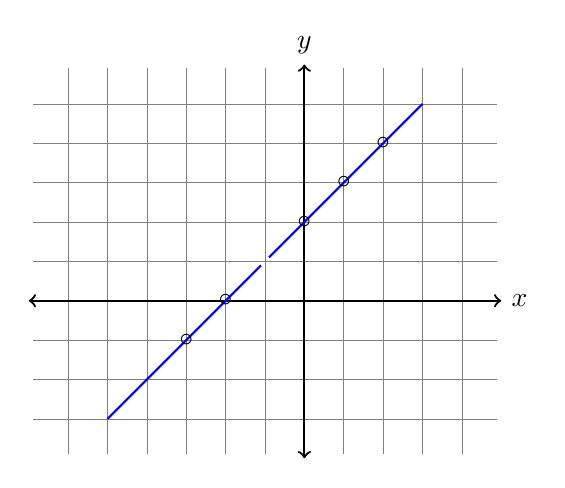
\begin{tikzpicture}[scale=0.5]
            \draw[step=1,gray,very thin] (-6.9,-3.9) grid (4.9,5.9);
            \draw[<->,thick] (-7, 0) -- (5, 0) node[right] {$x$};
            \draw[<->,thick] (0, -4) -- (0, 6) node[above] {$y$};

            \draw[domain=-5:-1.1, smooth, variable=\x, thick, blue] plot ({\x}, {(\x+2)});
            \draw[domain=-0.9:3, smooth, variable=\x, thick, blue] plot ({\x}, {(\x+2)});

            \foreach \Point in {(-3,-1), (-2,0), (0,2), (1,3), (2,4)}{
                \node at \Point {$\circ$};
            }
        \end{tikzpicture}
    \end{center}
\end{document}
